\documentclass[a4paper,12pt]{article}

\usepackage{Packages}
\usepackage{subfigure}
\usepackage{amsmath}


\begin{document}
\begin{titlepage}

\begin{center}

% Upper part of the page. The '~' is needed because \\
% only works if a paragraph has started.

\includegraphics[width=0.6\textwidth]{./Figures/TUe}~\\[2cm]


%\vspace*{10cm}

% Title
\HRule \\[0.4cm]
{ \huge \bfseries 2IMM20 - Foundations of datamining\\[0.3cm] }
\HRule \\[1.5cm]
\textbf{Assignment 2}


% Author and supervisor

\vfill

\begin{table}[h]
\begin{tabular}{ll}
\textbf{Students:} & \\
Joris van der Heijden & (0937329)\\
Bram van der Pol & (0780042)\\

\\
\textbf{Email addresseses:} & \\
j.j.m.v.d.heijden@student.tue.nl \\
a.f.v.d.pol@student.tue.nl \\
\\
\textbf{Supervisors:} &\\
Dr.ir. Joaquin Vanschoren
\\

%\textbf{Supervisors:} & \\
%Dr. M.Holenderski \\
\end{tabular}
\end{table}



% Bottom of the page
\large
{ Eindhoven, \today}

\end{center}


\end{titlepage}
 %included in part 1

\tableofcontents %included in part 1




\section{1. Moneyball}
\subsection{1.1}

{\it Visually explore the data. Plot the distribution of each feature (e.g. histograms), as well as the target. Visualize the dependency of the target on each feature (use a 2d scatter plot). Is there anything that stands out? Is there something that you think might require special treatment?
- Feel free to create additional plots that help you understand the data
- Only visualize the data, you don't need to change it (yet)} \\

The first column of figures shows the histograms of each column of the data in X. 
The second column shows the relationship between y and x. 

*Is there anything that stands out? Is there something that you think might require special treatment?*

The dataset containts missing values in column 9,10, 12 and 13 so the data set must first be pre-processed to visualize it. In order the scatterplot and histogram for the relevant features the NaN value were removed.
Beside the NaN the data the figures that do not show a clear distrubution are: 1, 8, 10 and 11, so these features may need further investigation as well. The relevant plots are visible in figure \ref{fig:scatter_hist}.\\

\begin{figure}

\centering    
\subfigure{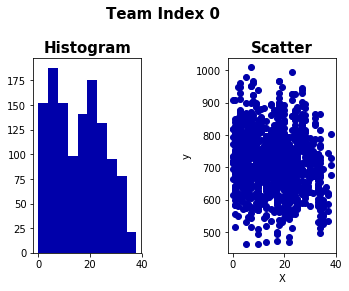
\includegraphics[width=40mm]{./Figures_1/output_5_141}}
\subfigure{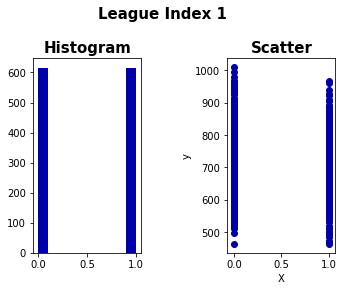
\includegraphics[width=40mm]{./Figures_1/output_5_142}}
\subfigure{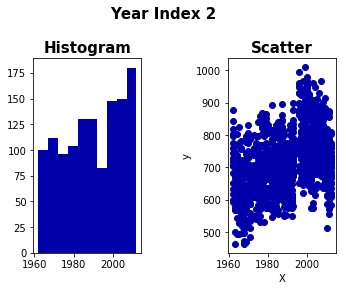
\includegraphics[width=40mm]{./Figures_1/output_5_143}}

\subfigure{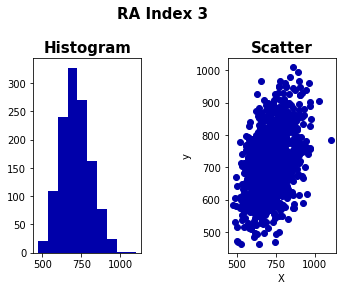
\includegraphics[width=40mm]{./Figures_1/output_5_144}}
\subfigure{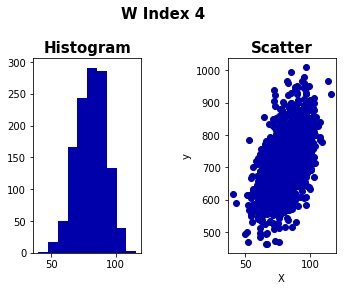
\includegraphics[width=40mm]{./Figures_1/output_5_145}}
\subfigure{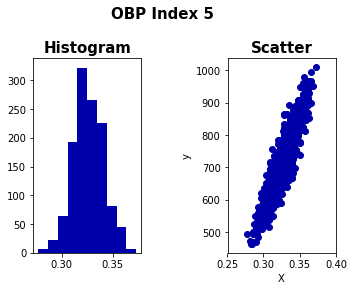
\includegraphics[width=40mm]{./Figures_1/output_5_146}}

\subfigure{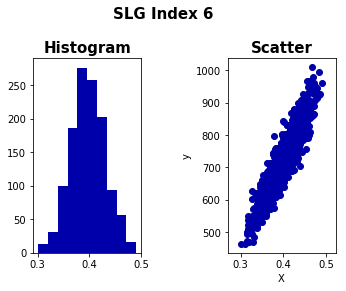
\includegraphics[width=40mm]{./Figures_1/output_5_147}}
\subfigure{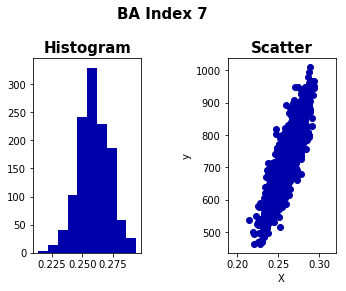
\includegraphics[width=40mm]{./Figures_1/output_5_148}}
\subfigure{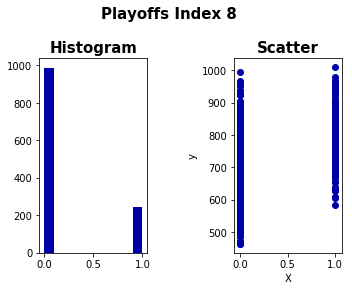
\includegraphics[width=40mm]{./Figures_1/output_5_149}}

\subfigure{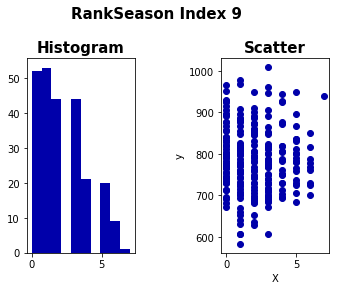
\includegraphics[width=40mm]{./Figures_1/output_5_150}}
\subfigure{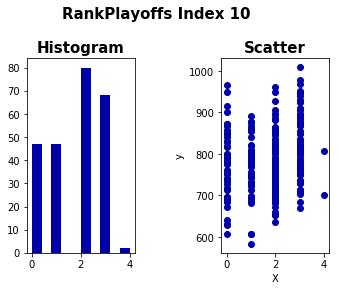
\includegraphics[width=40mm]{./Figures_1/output_5_151}}
\subfigure{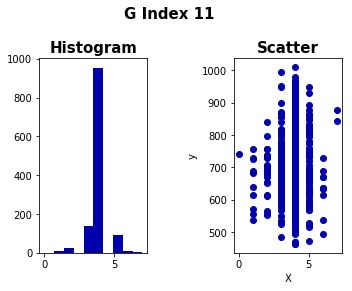
\includegraphics[width=40mm]{./Figures_1/output_5_152}}

\subfigure{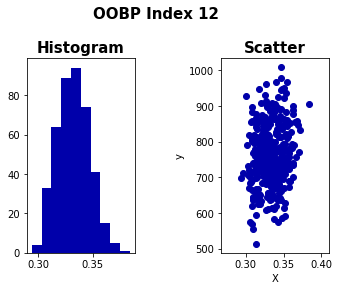
\includegraphics[width=40mm]{./Figures_1/output_5_153}}
\subfigure{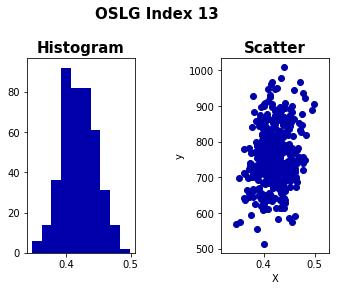
\includegraphics[width=40mm]{./Figures_1/output_5_154}}

\caption{Histograms and scatter plots of Moneyball features}
\label{fig:scatter_hist} %label altijd na caption..

\end{figure}

\subsection{1.2}
{\it Compare all linear regression algorithms that we covered in class (Linear Regression, Ridge, Lasso and ElasticNet), as well as kNN. Evaluate using cross-validation and the $R^2$ score, with the default parameters. Does scaling the data with StandardScaler help? Provide a concise but meaningful interpretation of the results.
- Preprocess the data as needed (e.g. are there nominal features that are not ordinal?). If you don't know how to proceed, remove the feature and continue.}\\

All features which have missing data were removed from the featureset before any further analysis. This means 4 features are removed completely and 10 features are considered for model generation. We chose to remove the data instead of filling in missing values because we were not sure which strategy to use for filling the blanks, and we assumed that using 10 out of the 14 features would still be enough to obtain sufficiently good models.

Without scaling, LinearRegression returns the best score at 0.92 and an r2 of 0.95. The other regression algorithms return worse, but still acceptable scores, with one exception: KNN yields a score of 0.00 and an r2 score of only 0.2. Most likely there is an error in how the KNN algorithm is used here, but we were unable to pinpoint the issue.

Using StandardScaler has no effect on the LinearRegression scores, but all other algorithms have significantly higher scores compared to their counterparts where scaling was not used. Ridge now matches the scores of LinearRegression, and Lasso comes close as well losing by 0.01 point in the r2 score. ElasticNet scores are also improved, but the scores are not as high as the other three algorithms. The KNN score improves sleightly but is still a lot lower then is to be expected. \\

A table containing all scores is visible in Table \ref{table:score_table}

\begin{table}[]
\centering
\caption{scoring data for several linear regression algorithms}
\label{table:score_table}
\begin{tabular}{lllll}
                  &       &      &                       &                    \\
                  & score & r2   & score\_StandardScaler & r2\_StandardScaler \\
Linear Regression & 0.92  & 0.95 & 0.92                  & 0.95               \\
Ridge             & 0.84  & 0.89 & 0.92                  & 0.95               \\
Lasso             & 0.80  & 0.86 & 0.92                  & 0.94               \\
KNN               & 0.00  & 0.20 & 0.01                  & 0.63               \\
ElasticNet        & 0.80  & 0.86 & 0.87                  & 0.90              
\end{tabular}
\end{table}


\subsection{1.3}
{\it Do a default, shuffled train-test split and optimize the linear models for the degree of regularization ($alpha$) and choice of penalty (L1/L2). For Ridge and  Lasso, plot a curve showing the effect of the training and test set performance ($R^2$) while increasing the degree of regularization for different penalties. For ElasticNet, plot a heatmap $alpha \times l1\_ratio \rightarrow R^2$ using test set performance.
Report the optimal performance. Again, provide a concise but meaningful interpretation. What does the regularization do? Can you get better results?
- Think about how you get the L1/L2 loss. This is not a hyperparameter in regression.
- We've seen how to generate such heatmaps in Lecture 3.} \\

To optimize alpha, a CVGridSearch was used. For Ridge ans Lasso, a logscale containing 100 samples from [0.001-100] were used as alpha parameter. For Ridge regression, alpha=0.001 returns the highest score, while for Lasso regression alpha=0.004 yielded the maximum score. Ridge regression performs L2 regularization, while Lasso regression performs L1 regularization, where alpha influences the L2/L1 penalty respectively. It is interesting to observe that for low values of alpha, Ridge and Lasso perform almost identically, as can be oberved in figure \ref{fig:ridgelasso}. It is interesting to note that the Lasso curve closely resembles a Tikhonov regularization L curve. \\

\begin{figure}
\centering    
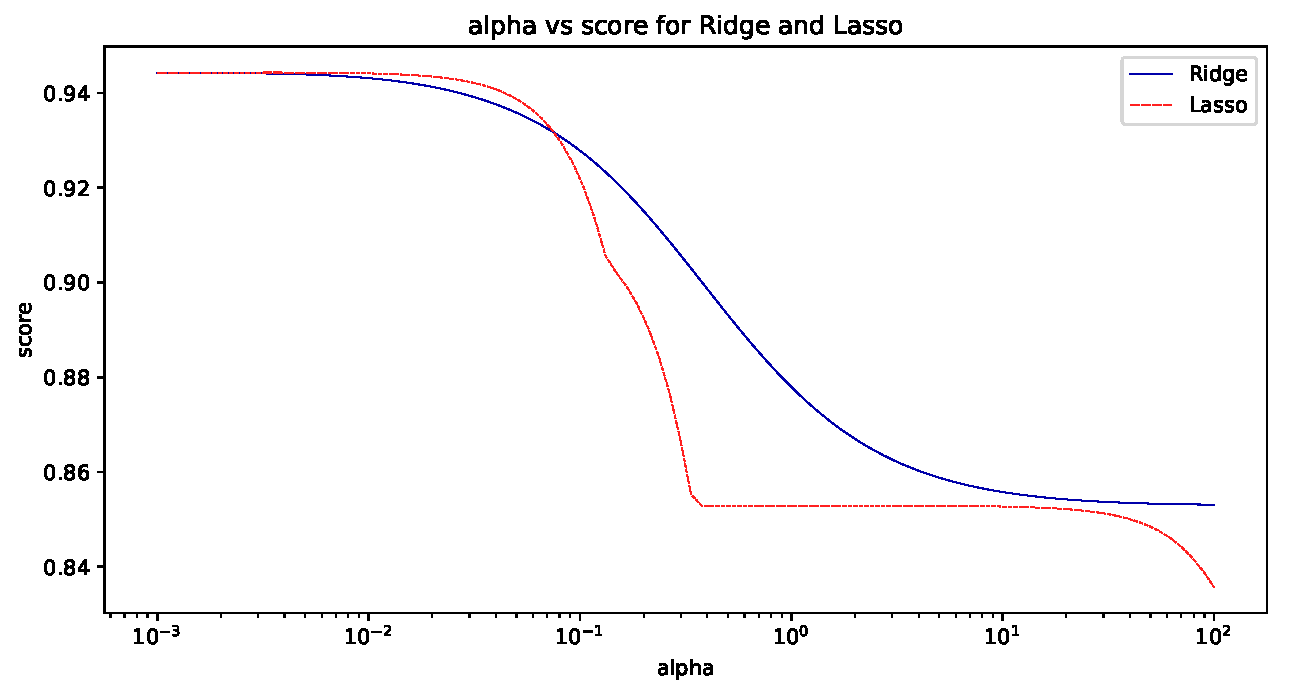
\includegraphics[width=120mm]{./Figures_1/ridgelasso}
\caption{score vs increasing regularization for Ridge and Lasso}
\label{fig:ridgelasso} %label altijd na caption..
\end{figure}

For ElasticNet 11 samples for the r1 ratio from [0-1]and 11 samples from[0.001-100] were used in the GridSearch. The highest scores are obtained with alpha=0.001, the lowest tested value for alpha, and an L1 ratio of 1. This is also clear from the heatmap in figure \ref{fig:elasticnet}. 
For KNN and LinearRegression no alpha hyperparameter exists, so these were not optimised.

\begin{figure}
\centering    
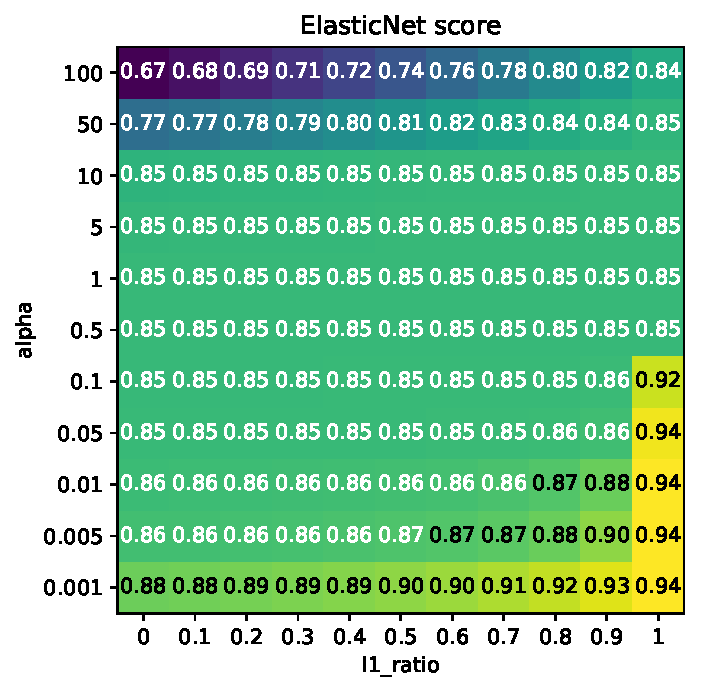
\includegraphics[width=100mm]{./Figures_1/elasticnet}
\caption{Histograms and scatter plots of Moneyball features}
\label{fig:elasticnet} %label altijd na caption..
\end{figure}

Higher scores might be obtained by trying a wider range of alpha values or using more samples per GridSearch. As seen in assignment 1.2, using a scaler may also lead to higher scores. A third option would be to use a RandomGridSearch which can try more values for alpha than the discrete steps used in a normal GridSearch. \\






\subsection{1.4}
{\it Visualize the coefficients of the optimized models. Do they agree on which features are
important? Compare the results with the feature importances returned by a RandomForest. Does it agree with the linear models? What would look for when scouting for a baseball player?}\\

LR, Ridge, Lasso and EN all seem to agree that the features with index 5 (OBP) is most important, followed closely by feature 6 (SLG). All other features have coefficients at least two orders of magnitude lower, so they hardly make a difference. Feature 5 (OBP) is On-Base Percentage, and feature 6 (SLG) is Slugging Percentage. However, the RandomForest paints a different picture entirely. While SLG and OBP are also relatively important according to the RandomForest, the Team, Year, BA, RA and W features get about the same importance scores. For all data, refer to table \ref{table:coefficients} and table \ref{table:rf}.

So, it seems deciding on important features to look for in Baseball players is not so clear cut. The linear models and RandomForest do agree on some features that are of lesser importance: League, Playoffs and G are features a scout does not need to pay attention to. \\

\begin{table}[]
\centering
\caption{Linear Regression coëfficients}
\label{table:coefficients}
\begin{tabular}{lllllllllll}
      & 0    & 1     & 2     & 3    & 4    & 5       & 6       & 7       & 8    & 11   \\
LR    & 0.07 & -4.56 & -0.33 & 0.27 & 2.61 & 2053.28 & 1203.09 & -119.03 & 1.43 & 4.08 \\
Ridge & 0.07 & -4.54 & -0.33 & 0.28 & 2.65 & 1997.63 & 1195.57 & -79.81  & 1.46 & 4.02 \\
Lasso & 0.07 & -4.49 & -0.32 & 0.28 & 2.74 & 1912.05 & 1172.60 & -0.00   & 1.47 & 3.91 \\
EN    & 0.07 & -4.54 & -0.33 & 0.27 & 2.64 & 2013.22 & 1193.86 & -74.72  & 1.45 & 4.05
\end{tabular}
\end{table}

\begin{table}[]
\centering
\caption{Random Forest feature importances}
\label{table:rf}
\begin{tabular}{lllllllllll}
   & 0      & 1      & 2      & 3      & 4      & 5      & 6      & 7      & 8      & 11     \\
RF & 0.1226 & 0.0311 & 0.1237 & 0.1398 & 0.1272 & 0.1213 & 0.1455 & 0.1312 & 0.0144 & 0.0433
\end{tabular}
\end{table}




\section{Nepalese character recognition}
\subsection{1}
{\it Evaluate k-Nearest Neighbors, Logistic Regression and RandomForests with their default
settings.
\begin{itemize}
\item{Take a stratified 10\% subsample of the data.}
\item{Use the default train-test split and predictive accuracy. Is predictive accuracy a good scoring measure for this problem?}
\item{Try to build the same models on increasingly large samples of the dataset (e.g. 10\%,
20\%,...). Plot the training time and the predictive performance for each. Stop when the
training time becomes prohibitively large (this will be different for different models).}
\end{itemize}
\textnormal{Because the logistic regression algorithm took more time than the k-Nearest and the Random Forest algorithm we made two figures; one based on maximum 20\% of the data and one based on maximum 6\% of the data. For this problem we used 75\% of the data to train the model and 25\% to validate the model.}

\begin{figure}[H]
\hfill
\makebox[\textwidth][c]{{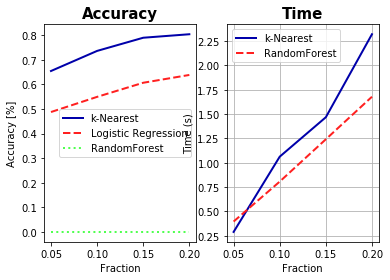
\includegraphics[width=12cm]{./Figures/output_15_1}}}
\hfill
\caption{Performance of the k-Nearest and Logistic regression algorithms. }
\label{Q21a}
\end{figure}

\begin{figure}[H]
\hfill
\makebox[\textwidth][c]{{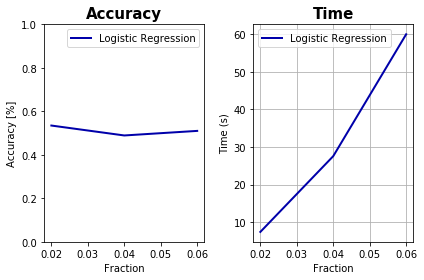
\includegraphics[width=12cm]{./Figures/output_15_3}}}
\hfill
\caption{Performance of the Logistic regression algorithm.}
\label{Q21b}
\end{figure}

\textnormal{Because the data size is sufficiently large the predictive accuracy is a good scoring measure. The characteristics of the k-Nearest and randomForest algorithm is shown in figure \ref{Q21a}. This figures shows that the accuracy of the models goes up when more data is used, which is expected. However figure \ref{Q21b} does not show this trend. We do not recommend this algorithm for this problem because of the time needed to train this algorithm and the accuracy of the model.}


\subsection{2}
{\it Optimize the value for the number of neighbors $k$ (keep $k < 50$) and the number of trees
(keep $n_{estimators} < 100$) on the stratified 10\% subsample. Use 10-fold crossvalidation and plot $k$ and $n_{estimators}$ against the predictive accuracy. Which value of $k, n_{estimators}$ should you pick?}\\

\begin{figure}[H]
\hfill
\makebox[\textwidth][c]{
\subfigure[]{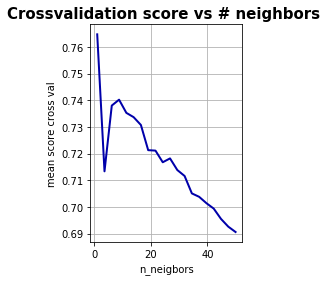
\includegraphics[width=6cm]{./Figures/output_17_1}}
\subfigure[]{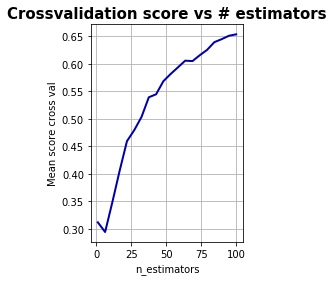
\includegraphics[width=6cm]{./Figures/output_17_3}}}
\hfill
\caption{}
\label{Q22}
\end{figure}
As can been seen in figure \ref{Q22} is that the number of neigbors should be set to 1 and the number of trees to 100. 

\subsection{3}
{\it For the RandomForest, optimize both $n_{estimators}$ and $max_{features}$ at the same time on the entire dataset. - Use a nested cross-validation and a random search over the possible values, and measure the accuracy. Explore how fine-grained this grid/random search can be, given your computational resources. What is the optimal performance you find? - Hint: choose a nested cross-validation that is feasible. Don’t use too many folds in the outer loop. - Repeat the grid search and visualize the results as a plot (heatmap) $n_{estimators}\cdot max_{features} \rightarrow ACC$ with ACC visualized as the color of the data point. Try to make the grid as fine as possible. Interpret the results. Can you explain your observations? What did you learn about tuning RandomForests?}
\begin{figure}[H]
\hfill
\makebox[\textwidth][c]{{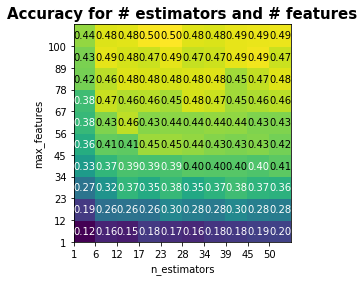
\includegraphics[width=12cm]{./Figures/output_19_1}}}
\hfill
\caption{Accuracy for the random forest for different maximum features and number of estimators numbers. This is done for 1\% of the total data set (due to the lack of computer power and time).}
\label{Q23}
\end{figure}
\textnormal{The finest grid which does not take too much time is in our case a 10x10 grid. This grid gives a good insight in the performance of the randomforest algorithm. We used only 1\% of the data because, unfortunately, the computing time was very large for 10\% of the data. This has a big influences on the results, however the characteristics of the algorithm can be examined. Figure \ref{Q23} shows that the number of trees in the forest. The optimal performance can be achieved by setting the number of estimators between 17 and 23 and the maximum features to 100. The more features that are available the better the data can be fitted, however overfitting the data can become a problem when the maximum number of features increases. The best number of trees does show a good accuracy for 50 number of trees. However the best accuracy can be increased by tuning the number of trees for a specific number of features.} 

\section{4}
\subsection{1}
{\it Do a bias-variance analysis of both algorithms. For each, vary the number of trees on a log scale from 1 to 1024, and plot the bias error (squared), variance, and total error (in one plot per algorithm). Interpret the results. Which error is highest for small ensembles, and which reduced most by each algorithm as you use a larger ensemble? When are both algorithms under- or over-fitting? Provide a detailed explanation of why random forests and gradient boosting behave this way. - See lecture 3 for an example on how to do the bias-variance decomposition - To save time, you can use a 10\% stratified subsample in your initial experiments, but show the plots for the full dataset in your report. In [ ]: from sklearn.model}

\begin{figure}[H]
\hfill
\makebox[\textwidth][c]{{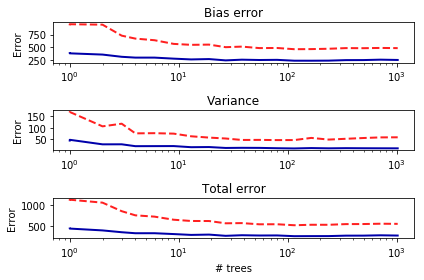
\includegraphics[width=12cm]{./Figures/output_24_1}}}
\hfill
\caption{RandomForests (blue lines )and Gradient Boosting (red dashed lines) as a function of the number of trees/ iterations.}
\label{Q41}
\end{figure}

\textnormal{The results shown in figure \ref{Q41} are not the results we expected. %We expected that the RandomForests and Gradient Boosting lines cross each other when the number of trees increases. This due to  
In general when the number of features/ iterations increased the model tend to overfit the data. However in this case each features is a pixel and the data is not overfitted. This also means that when the number of trees/ iterations increases all bias, variance and total errors goes down for this example. At the start both models are clearly under fitting because the number of total features of the image (1024) cannot be captured well. }

\subsection{2}
{\it A validation curve can help you understand when a model starts under- or overfitting. It plots both training and test set error as you change certain characteristics of your model, e.g. one or more hyperparameters. Build validation curves for gradient boosting, evaluated using AUROC, by varying the number of iterations between 1 and 500. In addition, use at least two values for the learning rate (e.g. 0.1 and 1), and tree depth (e.g. 1 and 4). This will yield at least 4 curves. Interpret the results and provide a clear explanation for the results. When is the model over- or underfitting? Discuss the effect of the different combinations learning rate and tree depth and provide a clear explanation.
While scikit-learn has a validation curve function, we'll use a modified version (below) that provides a lot more detail and can be used to study more than one hyperparameter. You can use a default train-test split.}

\textnormal{We added the $clf.fit(X\; train,y\; train)$ function before the Gradient boosting algorithm in order to make sere estimator was defined. The result is shown in figure \ref{Q41a} and figure \ref{Q41b}.}
 
\begin{figure}[H]
\hfill
\makebox[\textwidth][c]{{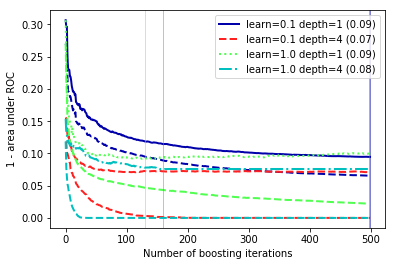
\includegraphics[width=12cm]{./Figures/output_26_3}}}
\hfill
\caption{Compute Receiver operating characteristic score for different hyperparameters for the gradient boosting algorithm. The lines in the legend is the training accuracy, the other lines show the test accuracy. }
\label{Q41a}
\end{figure}
Figure \ref{Q41a} clearly shows the underfitting when the number of boosting iterations are small. The convergence rate for the learning rate of 1 is clearly faster than for 0.1. The tree depth also has a big influence on the convergence rate, see the light blue and red lines. More features can be captured in the model so the model can captures the model more accurately. The expected overfitting of the data (the increase of the 1-ROC value) does not happen for 500 iterations so therefore we made an example for 5000 iterations, figure \ref{Q41b}. 
\begin{figure}[H]
\hfill
\makebox[\textwidth][c]{{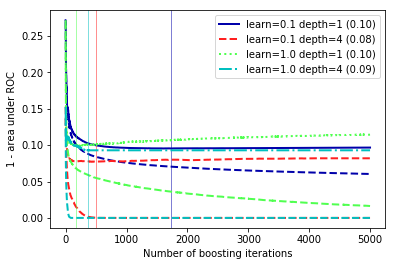
\includegraphics[width=12cm]{./Figures/output_26_2}}}
\hfill
\caption{Compute Receiver operating characteristic score for different hyperparameters for the gradient boosting algorithm. The number of iterations is set to 5000 to show possible overfitting characteristics.}
\label{Q41b}
\end{figure}

Overfitting of the data is not clearly visible even for 5000 iterations. 


\section{Appendix}
All code is availible on request by mailing one of the authors. Furthermore, all data is submitted in a "juptyter notebook" file as well as in a pdf version of that notebook. However, this PDF version is not entirely up to date as PDF generation broke somehow just before submission.

\end{document}
